\documentclass[titlepage,11pt]{article}
\usepackage{comment}
\usepackage{enumitem}
\usepackage{transparent} % Untuk transparansi gambar
\usepackage{listings}
\usepackage{amsmath}
\usepackage{graphicx}
\usepackage[font=small,labelfont=bf]{caption}
\usepackage[bahasa]{babel}
\usepackage{float}
\usepackage{verbatim}
\usepackage{graphicx,tabularx,multirow}
\usepackage{xcolor}
\usepackage[onehalfspacing]{setspace}
\usepackage{indentfirst}
\usepackage[
	allcolors=visigrey,
	colorlinks=true,
]{hyperref}
\usepackage[a4paper,left=2cm,right=2cm]{geometry}
% Pengaturan kutipan artikel
\usepackage[style=ieee, backend=biber]{biblatex}
%Code listing style pak akok
\definecolor{codegreen}{rgb}{0,0.6,0}
\definecolor{codegray}{rgb}{0.5,0.5,0.5}
\definecolor{codepurple}{rgb}{0.58,0,0.82}
\definecolor{backcolour}{rgb}{0.95,0.95,0.92}

\usepackage{eso-pic} % Untuk menambahkan elemen ke seluruh halaman

\newcommand\BackgroundPic{
  \put(0,0){
    \parbox[b][\paperheight]{\paperwidth}{
      \vfill
      \centering
      \transparent{0.1}
      
\includegraphics[width=0.4\paperwidth,keepaspectratio]{miot.png}
      \vfill
    }
  }
}

\newcommand\BackgroundAllPages{ \AddToShipoutPicture*{\BackgroundPic} }
\newcommand\BackgroundNone{ \ClearShipoutPicture } % hilangkan background

\lstdefinestyle{mystyle}{
	backgroundcolor=\color{backcolour}, commentstyle=\color{codegreen},
	keywordstyle=\color{magenta},
	numberstyle=\small\color{codegray},
	stringstyle=\color{codepurple},
	basicstyle=\ttfamily\footnotesize,
	breakatwhitespace=false,         
	breaklines=true,                 
	captionpos=t,                    
	keepspaces=true,                 
	numbers=left,                    
	numbersep=5pt,                  
	showspaces=false,                
	showstringspaces=false,
	showtabs=false,           
	frame = single,
	tabsize=2
}
\lstset{style=mystyle}

\definecolor{visigrey}{rgb}{.1,.15,.15}
\geometry{top=1cm,bottom=.5cm}
\savegeometry{titlepage}
\geometry{top=2cm,bottom=2cm}
\savegeometry{main}

\def\bspace{\(\qquad\qquad\qquad\)}
\usepackage[T1]{fontenc}
\usepackage[utf8]{inputenc}
\usepackage{tgheros}
\renewcommand*\familydefault{\sfdefault}

\setcounter{tocdepth}{6}

\def\autor{Laboratorium }
\def\lab{Multimedia dan Internet of Things}
\def\departemen{Departemen Teknik Komputer}
\def\institut{Institut Teknologi Sepuluh Nopember}
\def\praktikum{Laporan Sementara \\ Praktikum Jaringan Komputer}
\def\nama{Muhammad Zia Alhambra - 5024231059}
% Ubah Judul sesuai dengan modul
\def\judul{Modul Firewall \& NAT}
\def\tanggal{2025}
\begin{document}
% Ubah Bahasa sesuai dengan keinginan
\selectlanguage{bahasa}

\BackgroundNone
\def\headingtype{\bf \small}
\loadgeometry{titlepage}

\begin{titlepage}
	\centering
	\begin{tabularx}{\textwidth}{l@{\hskip 0pt}lX}
		\raisebox{-0.5\height}{
\includegraphics[width=3cm]{Cover/img/logodepart.png}} 
		& \raisebox{-0.5\height}{
\includegraphics[width=3cm]{Cover/img/miot.png}} 
		& \raggedleft
	\hfill
	\begin{minipage}{0.5\textwidth}
		\raggedleft
		{\emph{\headingtype \autor}} \\[-2pt]
		{\headingtype \lab} \\[-2pt]
		{\headingtype \departemen} \\[-2pt]
		{\headingtype \emph{\institut}}
	\end{minipage}

	\vspace{5cm}
	\end{tabularx}
	
	\vspace{5cm}
	{\Huge \bf \praktikum \par}
	
	\vspace{2cm}
	{\LARGE \bf \judul \par}
	
	\vspace{2cm}
	{\Large \nama \par}
	
	\vfill
	{\Large \tanggal \par}
	
	\vfill
	
\includegraphics[width=\textwidth]{Cover/img/footer.png}
\end{titlepage}

\loadgeometry{main}


\BackgroundAllPages
% Pilih Modul yang akan di build
\section{Langkah-Langkah Percobaan}
\begin{enumerate}
    \item Konfigurasi Router VPN PPTP PC dengan Router
    \begin{enumerate}
        \item Reset Konfigurasi Router lalu mausk ke winbox.
        \begin{center}
            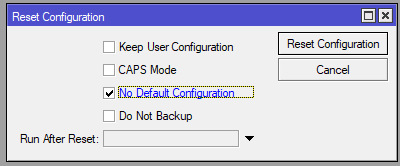
\includegraphics[scale=1]{P1/img/1 reset config.png}        
        \end{center}
        \item Konfigurasi DHCP Client (Koneksi Internet). Langkah ini bertujuan agar router mendapatkan koneksi internet dari sumber (ISP).
        \begin{itemize}
            \item  Buka menu IP > DHCP Client.
            \item Klik tombol + (Add) untuk menambahkan.
            \item Pada jendela baru:
            \item Interface: Pilih ether3 (atau interface yang terhubung ke sumber internet).
            \item Pastikan opsi "Use Peer DNS" dan "Use Peer NTP" tercentang.
            \item Klik Apply lalu OK. Router sekarang seharusnya sudah mendapatkan alamat IP dari ISP.
        \end{itemize}
        \begin{center}
            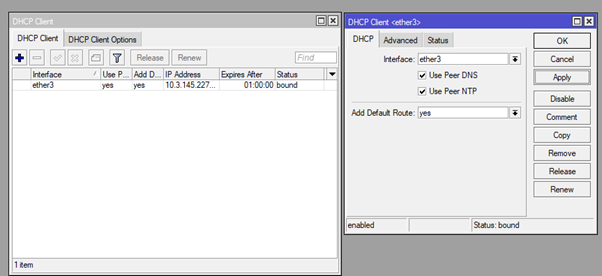
\includegraphics[scale=0.7]{P1/img/2 Konfigurasi DHCP Client.png}        
        \end{center}
        \item Konfigurasi Firewall NAT. Langkah ini sangat penting agar semua perangkat di jaringan lokal (ether3) dapat terhubung ke internet.
        \begin{itemize}
            \item Buka menu IP > Firewall.
            \item Pindah ke tab NAT.
            \item Klik tombol + (Add) untuk membuat aturan baru.
            \item Pada tab General:
            \item Chain: srcnat
            \item Out. Interface: ether3 (interface yang terhubung ke internet)
            \item Pindah ke tab Action:
            \item Action: masquerade
            \item Klik Apply lalu OK.
        \end{itemize}
        \begin{center}
            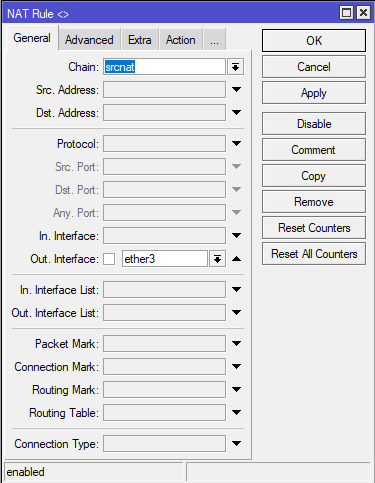
\includegraphics[scale=0.5]{P1/img/3 Konfigurasi DHCP Client 1.png}        
        \end{center}
        \begin{center}
            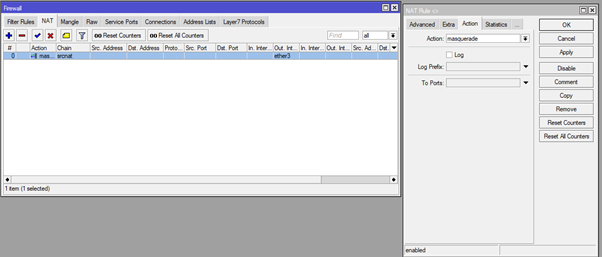
\includegraphics[scale=0.7]{P1/img/4 Hasil Konfigurasi DHCP Client.png}        
        \end{center}
        \item Konfigurasi Alamat IP Lokal (LAN). Tambahkan alamat IP untuk jaringan lokal yang akan terhubung ke ether1
        \begin{itemize}
            \item Buka menu IP > Addresses.
            \item Klik tombol + (Add).
            \item Isi form sebagai berikut:
            \item Address: 192.168.10.2/24
            \item Interface: ether1
            \item Klik Apply lalu OK.
        \end{itemize}
        \begin{center}
            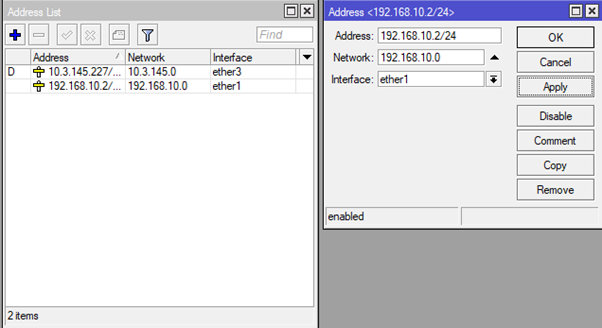
\includegraphics[scale=0.7]{P1/img/5 Konfigurasi Alamat IP Lokal (LAN).png}        
        \end{center}
        \item Konfigurasi DHCP Server (Distribusi IP ke Klien). Atur server DHCP agar perangkat klien (laptop/PC) yang terhubung ke ether1 mendapatkan IP secara otomatis.
        \begin{itemize}
            \item Buka menu IP > DHCP Server.
            \item Klik tombol "DHCP Setup".
            \item DHCP Server Interface: Pilih ether1 > Next.
            \item DHCP Address Space: Verifikasi network 192.168.10.0/24 > Next.
            \item Gateway for DHCP Network: Verifikasi gateway 192.168.10.2 > Next.
            \item Addresses to Give Out: Tentukan rentang IP untuk klien, misalnya 192.168.10.1-192.168.10.254 > Next.
            \item DNS Servers: Alamat DNS akan terisi otomatis dari DHCP Client (sumber internet). Klik Next.
            \item Lease Time: Atur durasi sewa IP, misalnya 00:10:00 > Next.
            \item Jika muncul pesan "Setup has completed successfully", klik OK.
        \end{itemize}
        \begin{center}
            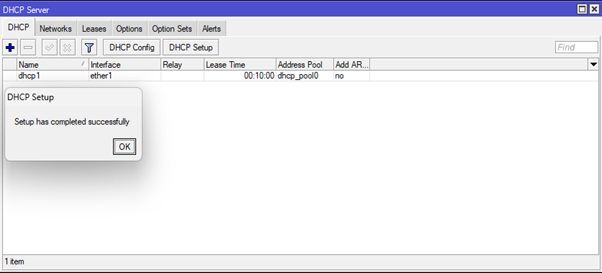
\includegraphics[scale=0.7]{P1/img/6 Konfigurasi DHCP Server.png}        
        \end{center}
        \item Mengaktifkan Proxy ARP. Ubah mode ARP pada interface yang terhubung ke PC2 untuk membantu proses bridging dan routing. Buka menu Interfaces. Klik dua kali pada interface ether1. Pada tab General, ubah pengaturan ARP dari enabled menjadi proxy-arp. Klik OK.
        \begin{center}
            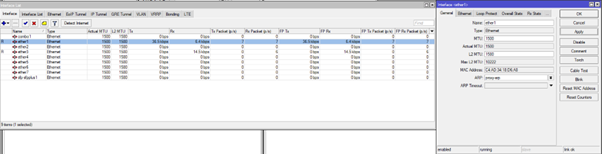
\includegraphics[scale=0.9]{P1/img/7. Mengaktifkan Proxy ARP '.png}        
        \end{center}
        \item Konfigurasi PPTP Server VPN a. Mengaktifkan PPTP Server. Buka menu PPP. Pada tab Interface, klik tombol "PPTP Server". Centang kotak Enabled. Klik OK.
        \begin{center}
            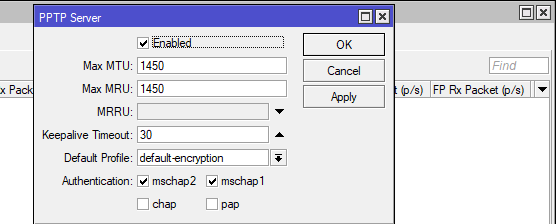
\includegraphics[scale=0.9]{P1/img/8 Konfigurasi Mengaktifkan PPTP Server.png}        
        \end{center}
        \item Membuat User \& Password (Secrets) Kredensial ini akan digunakan oleh klien untuk login VPN.
        \begin{itemize}
            \item Di jendela PPP, buka tab Secrets.
            \item Klik tombol + (Add) untuk menambah user baru.
            \item Isi form sebagai berikut:
            \item Name: mahasiswa
            \item Password: praktikum123
            \item Service: pptp
            \item Local Address: 192.168.10.2 (IP ini akan menjadi IP gateway tunnel untuk klien)
            \item Remot Address: 192.168.10.5
            \item Klik OK.
        \end{itemize}
        \begin{center}
            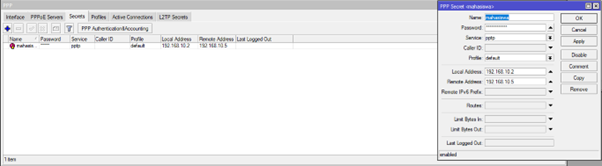
\includegraphics[scale=0.9]{P1/img/9 Konfigurasi Membuat User & Password (Secrets) Kredensial.png}        
        \end{center}
        \item Konfigurasi PPTP Client di Laptop (Windows). Sekarang, siapkan laptop untuk terhubung ke PPTP Server yang telah dibuat.
        \begin{itemize}
            \item Buka Settings → Network \& Internet → VPN.
            \item Klik "Add a VPN connection".
            \item Isi detail koneksi:
            \item VPN provider: Pilih Windows (built-in).
            \item Connection name: VPN Router Praktikum
            \item Server name or address: Masukkan IP Address ether3 yang didapat dari DHCP Client.
            \item VPN type: Point to Point Tunneling Protocol (PPTP).
            \item Type of sign-in info: User name and password.
            \item User name: mahasiswa
            \item Password: praktikum123
            \item Centang "Remember my sign-in info" dan klik Save.
            \item Hubungkan ke VPN yang baru dibuat.
        \end{itemize}
        \begin{center}
            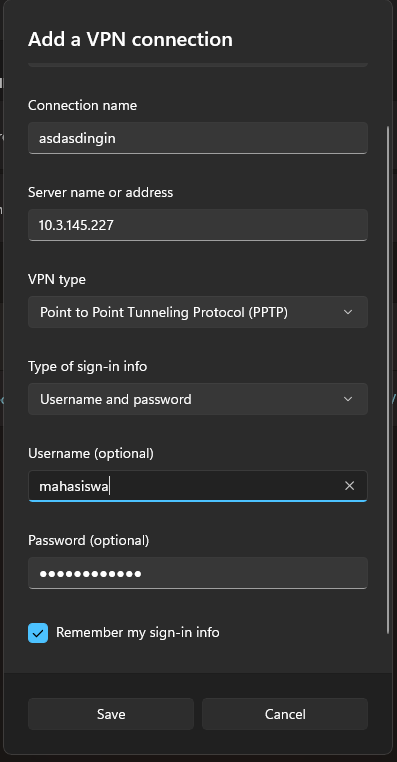
\includegraphics[scale=0.5]{P1/img/10 Konfigurasi PPTP Client di Laptop (Windows).png}
            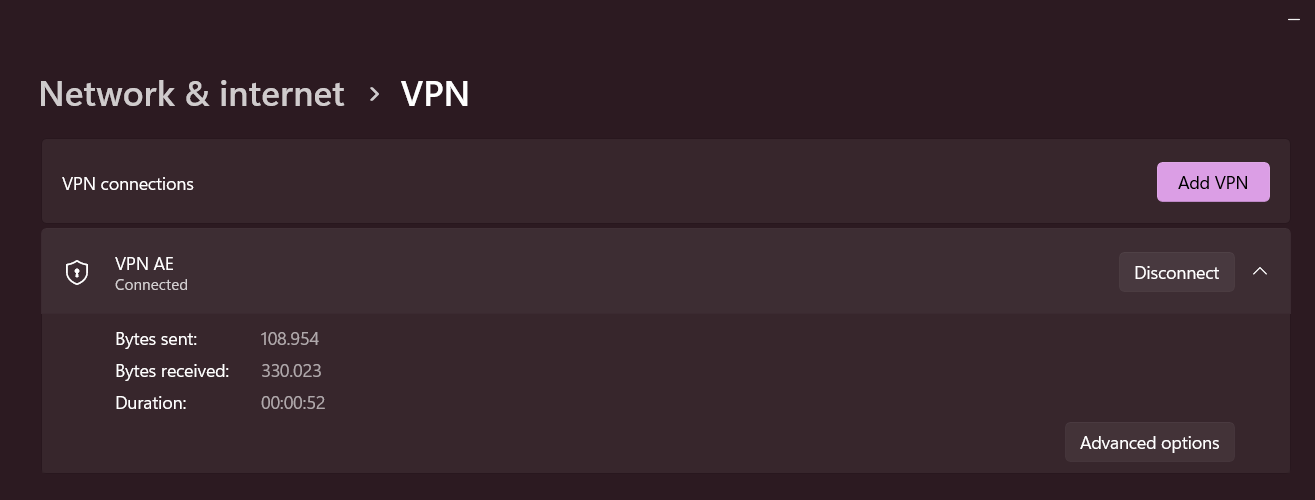
\includegraphics[scale=0.3]{P1/img/12 Hasil Konfigurasi PPTP Client di Laptop (Windows).png}        
        \end{center}
        \item Verifikasi koneksi dengan melakukan ping antar PC.
        \item \begin{center}
            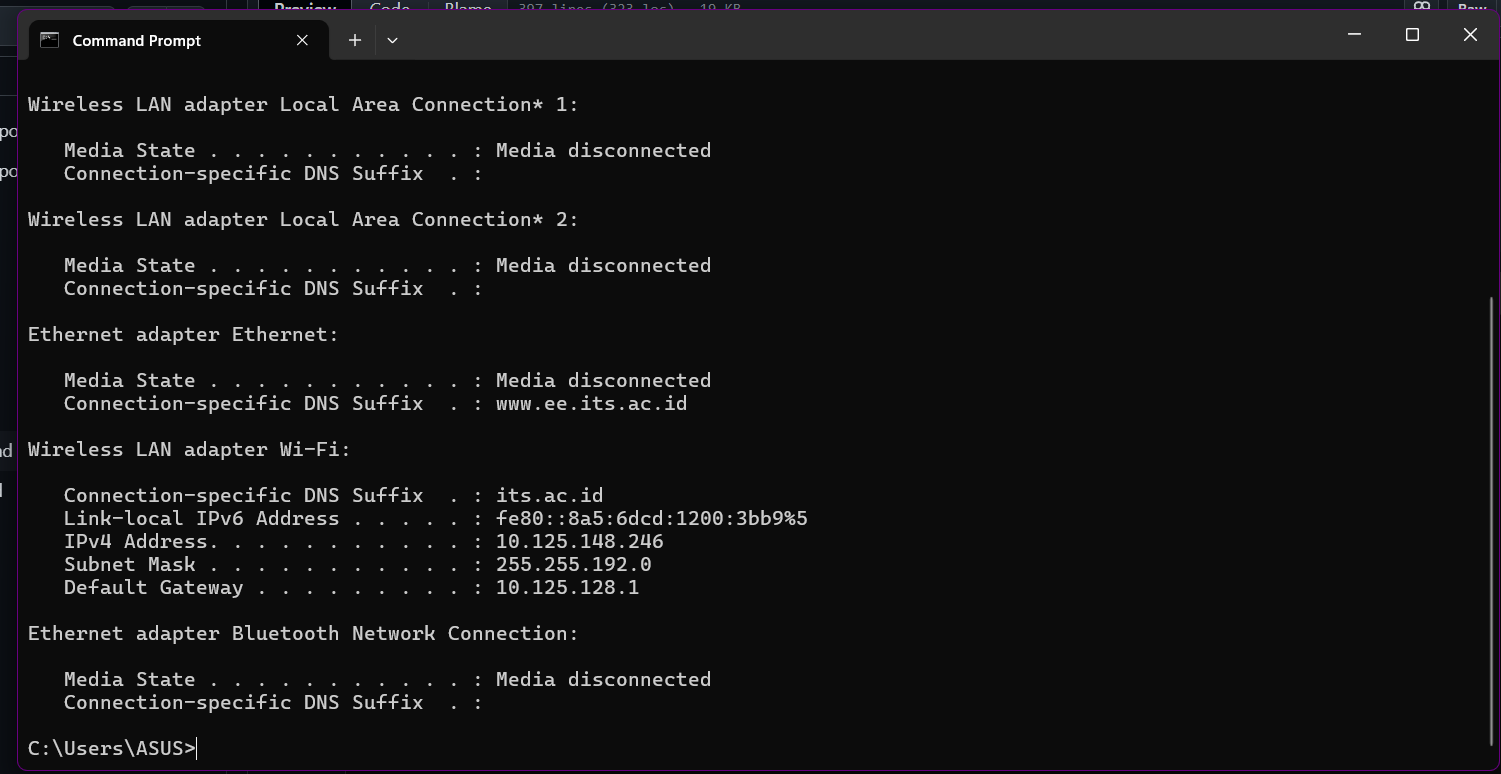
\includegraphics[scale=0.3]{P1/img/13 ipconfig.png}
            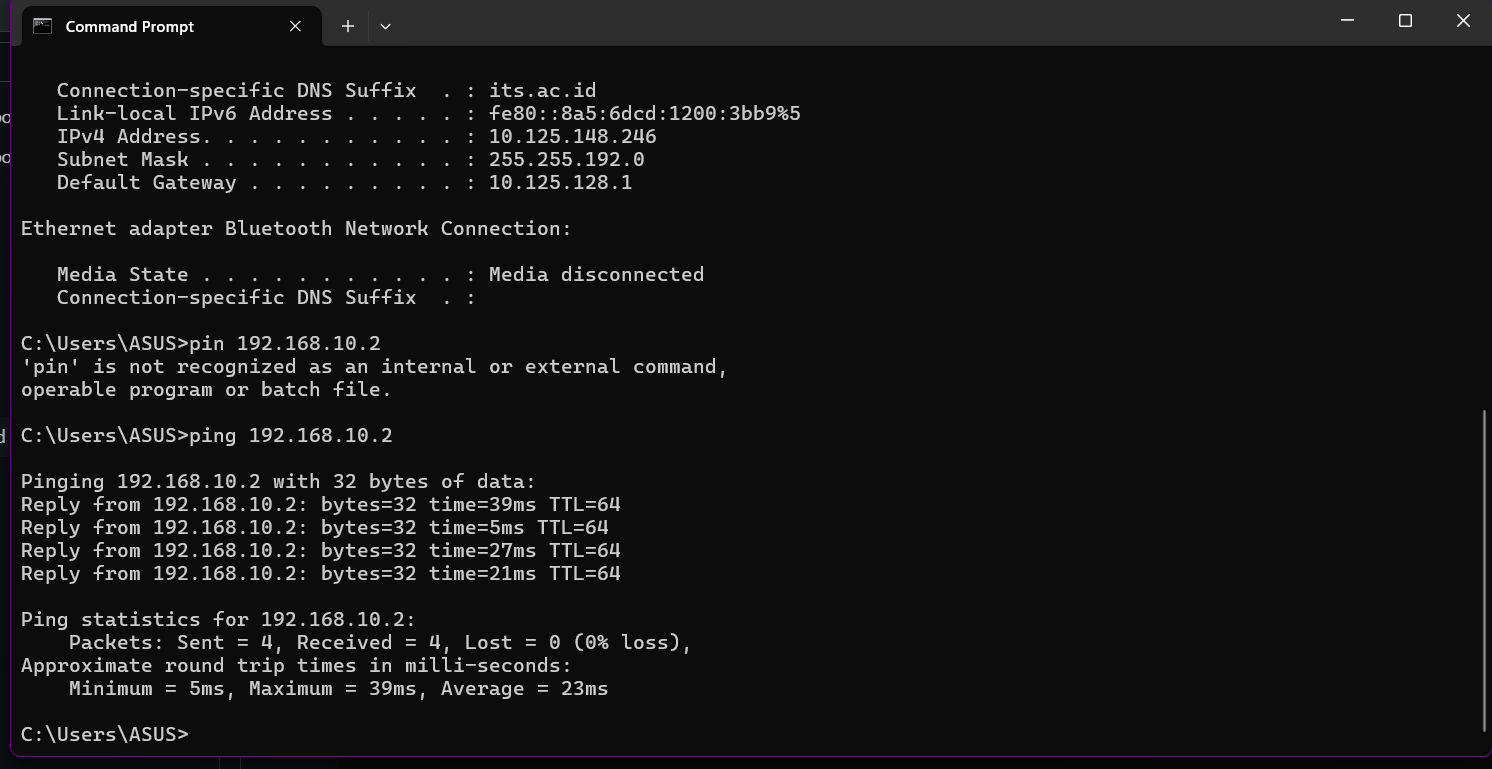
\includegraphics[scale=0.3]{P1/img/14 ping 192.168.10.2.png}    
            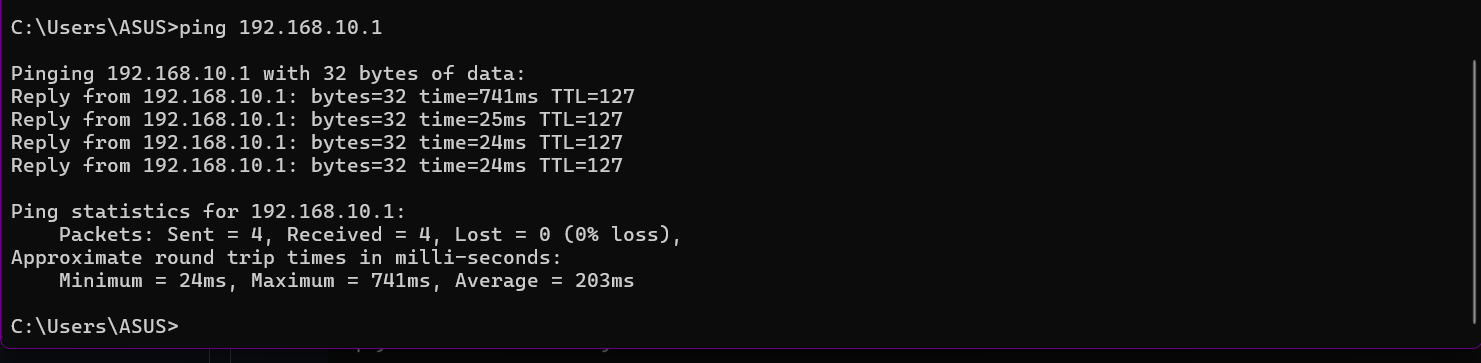
\includegraphics[scale=0.3]{P1/img/15 ping 192.168.10.1.png}       
        \end{center}

    \end{enumerate}
    \item Konfigurasi QOS PC dengan Router (Router Tidak perlu di Reset)
    \begin{enumerate}
        \item Membuat Aturan Simple Queue Langkah ini bertujuan untuk membatasi kecepatan upload dan download untuk klien yang terhubung ke jaringan. Buka menu Queues di Winbox. Di dalam tab Simple Queues, klik tombol + (Add) untuk membuat aturan baru.
        \begin{itemize}
            \item Pada tab General, konfigurasikan sebagai berikut:
            \item Name: Beri nama yang deskriptif, contoh: Limit-PC-Klien
            \item Target: Masukkan alamat IP atau network klien yang ingin dibatasi. Contoh: 192.168.10.0/24 (untuk membatasi semua klien di jaringan ether1 yang dibuat sebelumnya).
            \item Max Limit (Upload): 1M
            \item Max Limit (Download): 1M
            \item Klik Apply lalu OK.
        \end{itemize}
        \begin{center}
            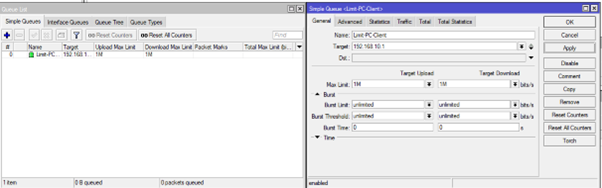
\includegraphics[scale=0.9]{P1/img/1 Membuat Aturan Simple Queue.png}        
        \end{center}
        \item Memantau Penggunaan Traffic. Anda dapat melihat lalu lintas data secara real-time untuk memastikan queue berfungsi.
        \begin{itemize}
            \item Buka kembali menu Queues dan pilih tab Simple Queues.
            \item Klik dua kali pada aturan queue yang baru saja Anda buat (Limit-PC-Klien).
            \item Pindah ke tab Traffic. Di sini, Anda akan melihat grafik real-time untuk upload dan download yang melewati aturan ini saat klien sedang menggunakan internet.
        \end{itemize}
        \begin{center}
            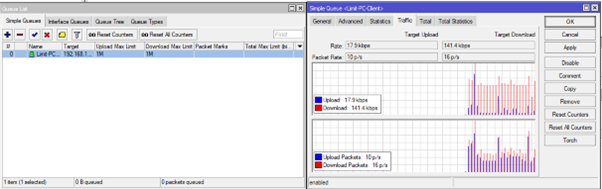
\includegraphics[scale=0.9]{P1/img/2 Memantau Penggunaan Traffic.png}        
        \end{center}
        \item Pengujian Efektivitas Queue. Lakukan pengujian untuk membandingkan kecepatan internet sebelum dan sesudah queue diaktifkan.
        \begin{center}
            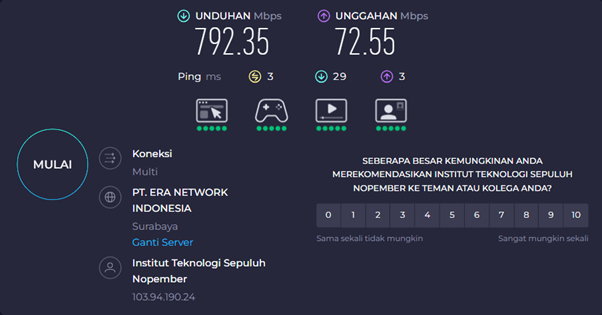
\includegraphics[scale=0.9]{P1/img/3 A. Tes Saat Queue Tidak Aktif.png}        
            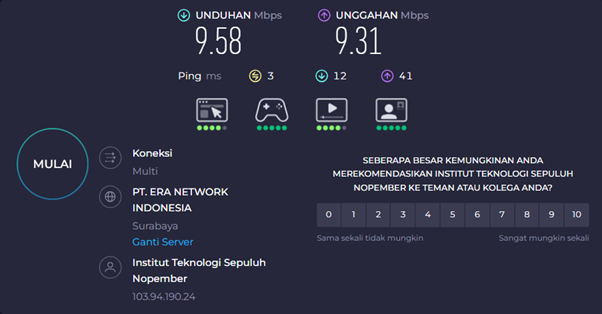
\includegraphics[scale=0.9]{P1/img/4 B Tes Saat Queue Aktif.png}
        \end{center}
    \end{enumerate}
\end{enumerate}
\section{Analisis Hasil Percobaan}
\begin{enumerate}
    \item Konfigurasi Router VPN PPTP PC dengan Router
     
    Percobaan dalam penerapan VPN menggunakan PPTP menunjukkan hasil yang memuaskan. Keberhasilan ini dibuktikan melalui pengujian konektivitas berupa perintah ping dari PC klien yang terhubung melalui VPN ke gateway router dan perangkat lain di jaringan internal. Temuan ini mendukung teori bahwa protokol PPTP mampu membentuk saluran virtual yang aman, memungkinkan klien eksternal untuk terhubung seolah-olah menjadi bagian dari jaringan lokal. Salah satu elemen penting dalam keberhasilan ini adalah konfigurasi NAT masquerade yang tepat, yang membuat router dapat diakses dari jaringan luar, serta ketepatan informasi login di bagian Secrets untuk proses autentikasi. Selama pengujian berlangsung, tidak ditemukan kendala maupun error.
    
    \item Konfigurasi QOS PC dengan Router
    
    Dalam uji coba fitur Quality of Service (QoS), penggunaan Simple Queue terbukti efektif dalam mengendalikan bandwidth. Hasil yang diperoleh menunjukkan perbedaan signifikan pada kecepatan internet sebelum dan sesudah pengaturan queue diaktifkan. Ketika Simple Queue dijalankan, kecepatan unduhan dan unggahan klien dibatasi sesuai nilai Max Limit yang telah disetting, yaitu 1 Mbps. Temuan ini mendukung teori mengenai fungsi Simple Queue dalam pengaturan lebar pita. Keberhasilan implementasi bergantung pada keakuratan penetapan alamat Target dan nilai Max Limit. Kesalahan pada salah satu parameter dapat menyebabkan aturan tidak berjalan. Karena hasil yang diamati sesuai dengan pengaturan, maka percobaan dinyatakan berhasil.
\end{enumerate}
\section{Hasil Tugas Modul}
Topologi :

PC1 - Router 1 - Internet - Router 2 - PC2

Membuat simulasi jaringan menggunakan Cisco Packet Tracer yang menunjukkan konektivitas antar dua jaringan melalui protokol PPTP (Point-to-Point Tunneling Protocol).

\begin{enumerate}
    \item Buatlah sebuah simulasi jaringan di Cisco Packet Tracer dengan topologi sebagai berikut:
    \begin{itemize}
        \item Terdapat 2 buah Router yang terhubung satu sama lain menggunakan Protokol PPTP.
        \item Masing-masing Router memiliki 1 buah PC client
        \item Konfigurasikan koneksi antar kedua Router menggunakan PPTP VPN agar jaringan di kedua sisi dapat saling terhubung secara aman.
        \item Lakukan pengaturan IP pada masing-masing perangkat (Router dan PC).
    \end{itemize}
    \begin{center}
        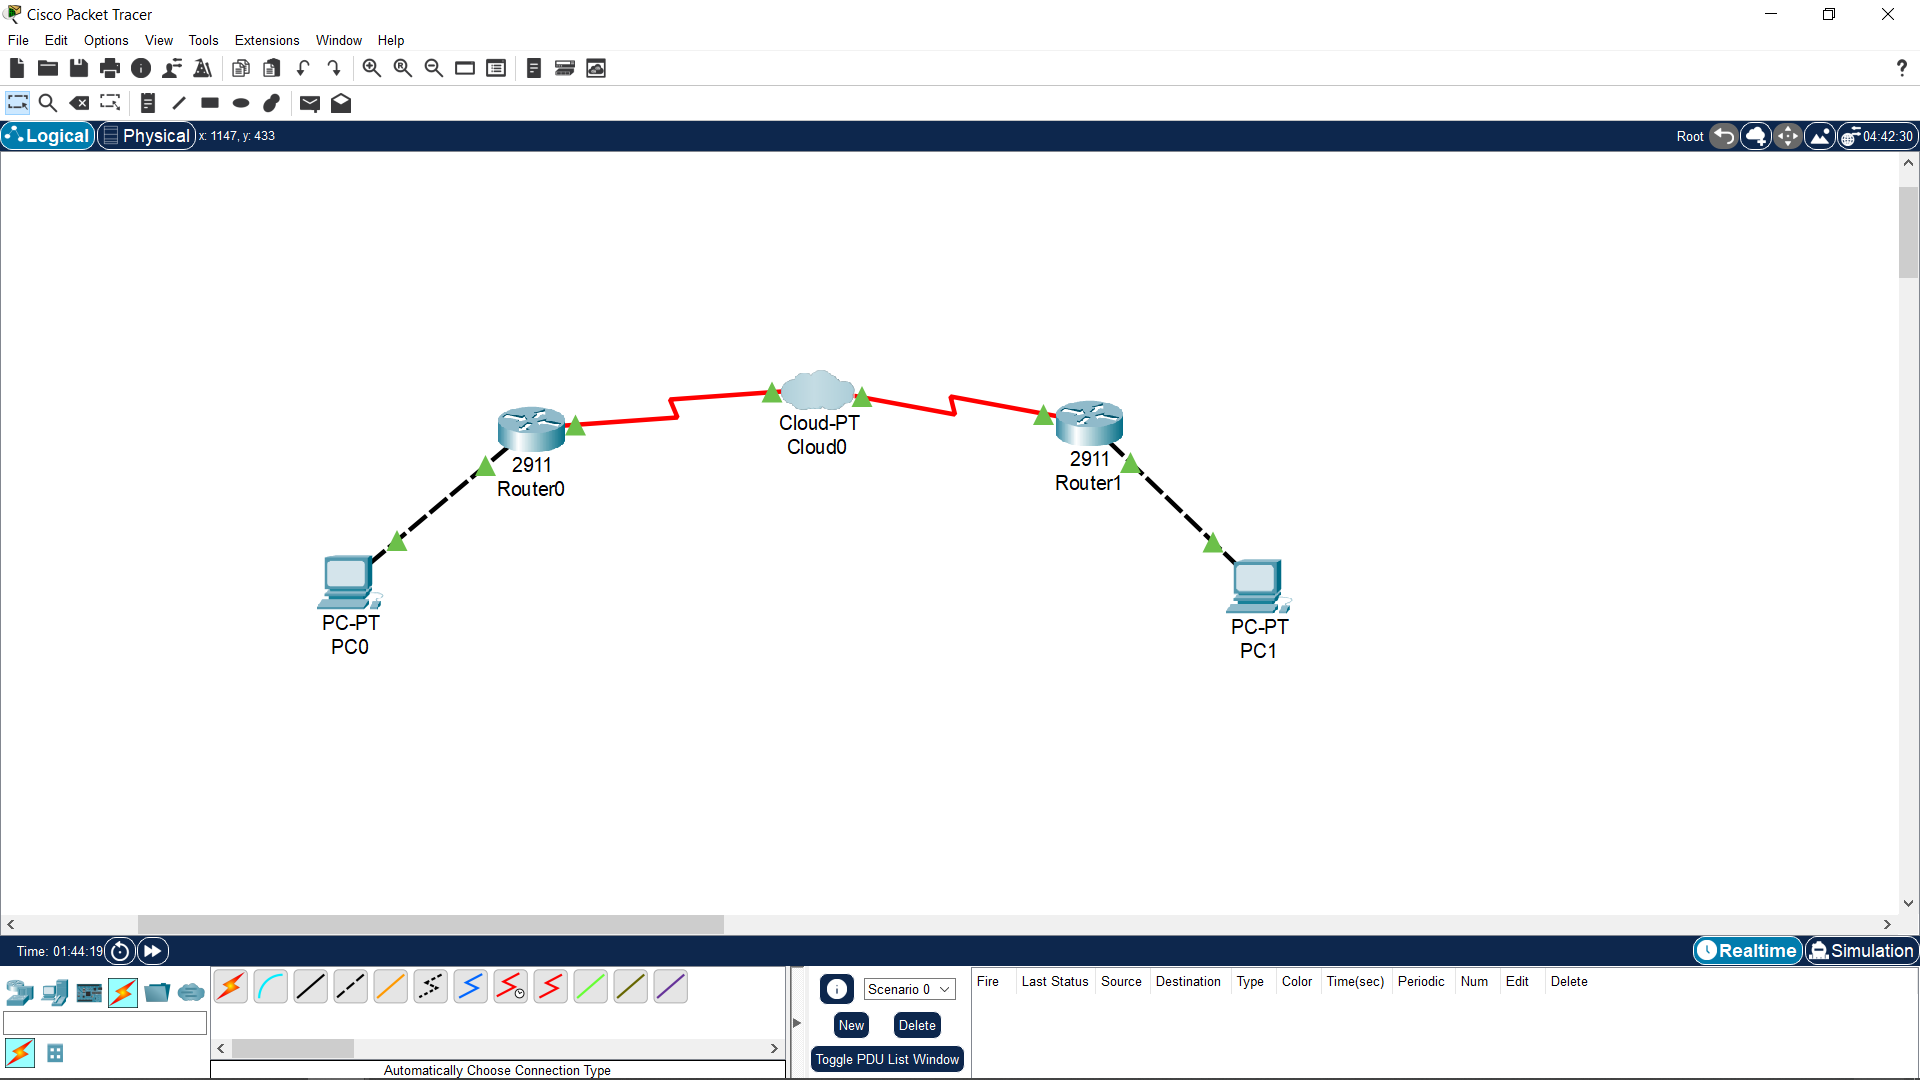
\includegraphics[scale=0.2]{P1/img/topologi.png}        
    \end{center}
    \item Pastikan setelah konfigurasi selesai:
    \begin{itemize}
        \item PC yang berada pada jaringan Router pertama dapat melakukan ping ke PC yang berada pada jaringan Router kedua, dan sebaliknya.
    \end{itemize}
    \begin{center}
        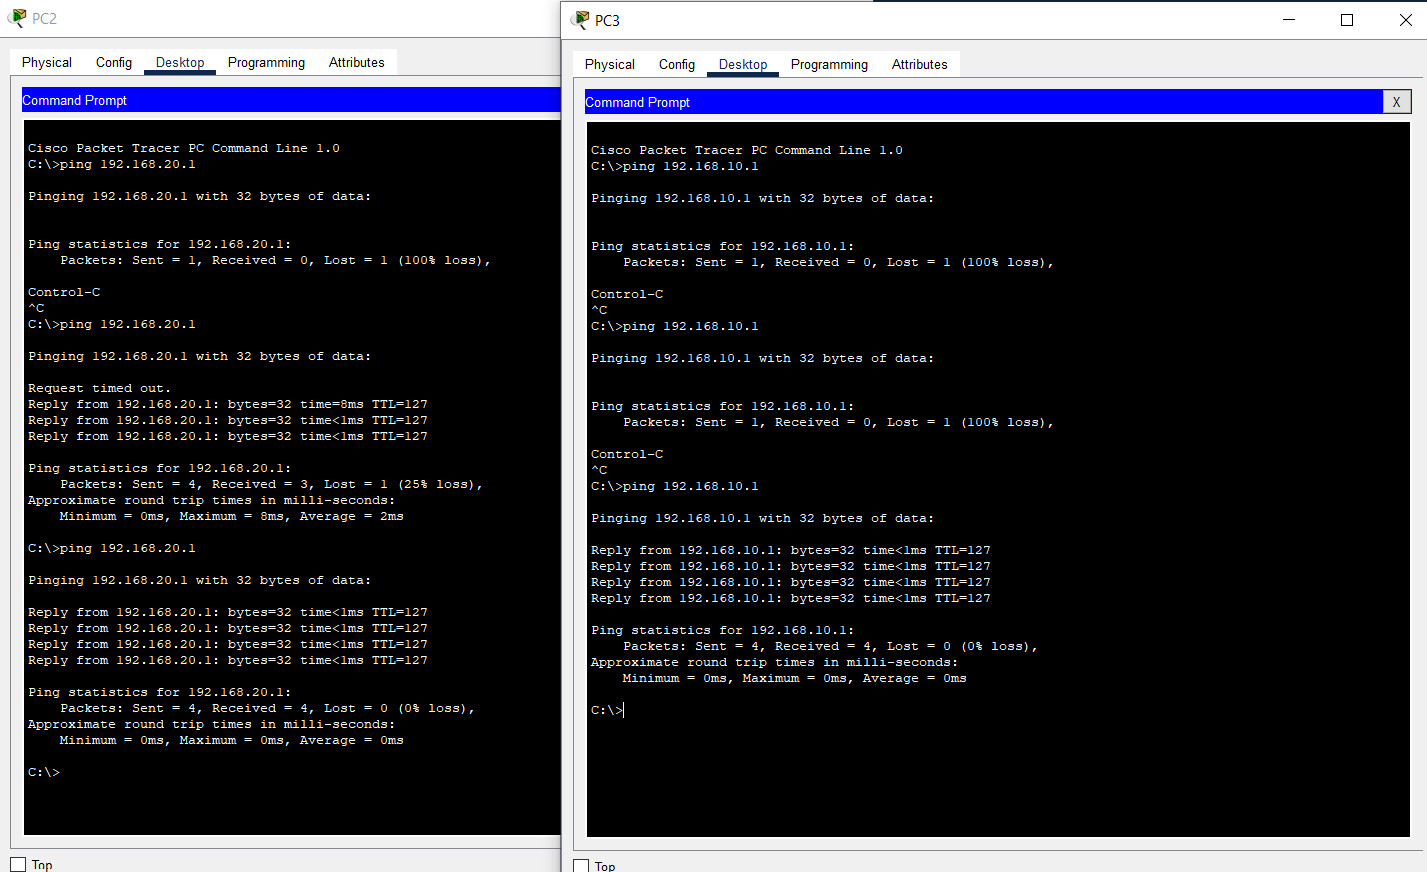
\includegraphics[scale=0.5]{P1/img/jarkom5-1.png}        
    \end{center}
    \item Masukan dalam laporan berikut :
    \begin{itemize}
        \item Topologi jaringan (screenshot dari Cisco Packet Tracer).
        \item Hasil pengujian konektivitas (ping test antar PC).
        \item Penjelasan singkat tentang fungsi PPTP dalam jaringan tersebut.
    \end{itemize}
    Penjelasan Singkat:

    PPTP (Point-to-Point Tunneling Protocol) berperan sebagai protokol untuk membentuk koneksi VPN (Virtual Private Network) yang aman antara dua jaringan yang terpisah secara geografis. Dalam topologi jaringan yang telah dirancang, PPTP dimanfaatkan untuk menciptakan terowongan virtual antara dua router, sehingga masing-masing jaringan lokal yang terhubung ke router tersebut dapat saling terhubung secara langsung dan aman, seolah-olah berada dalam satu jaringan lokal. Data yang ditransmisikan antara kedua jaringan akan melalui proses enkapsulasi dan dapat dienkripsi untuk menjaga kerahasiaan serta keutuhan informasi saat melewati jaringan publik seperti internet.

\end{enumerate}
\section{Kesimpulan}
Berdasarkan hasil pengujian yang telah dilakukan, konfigurasi VPN berbasis protokol PPTP berhasil diimplementasikan sesuai dengan target. Dua jaringan lokal yang terhubung melalui router mampu berkomunikasi dengan aman seakan berada dalam satu jaringan internal yang sama. Seluruh tahapan konfigurasi—mulai dari penetapan IP, DHCP, NAT, hingga pembuatan akun pengguna dan aktivasi layanan VPN—berjalan dengan lancar dan menghasilkan koneksi yang stabil. Hasil pengujian menunjukkan bahwa perangkat dari masing-masing jaringan dapat saling melakukan ping tanpa gangguan, mengindikasikan bahwa koneksi VPN aktif dan bekerja sebagaimana mestinya. Selain itu, fitur QoS juga berhasil diaktifkan untuk mengatur penggunaan bandwidth sesuai batas yang telah ditentukan.

\section{Lampiran}
\subsection{Dokumentasi saat praktikum}
    \begin{center}
        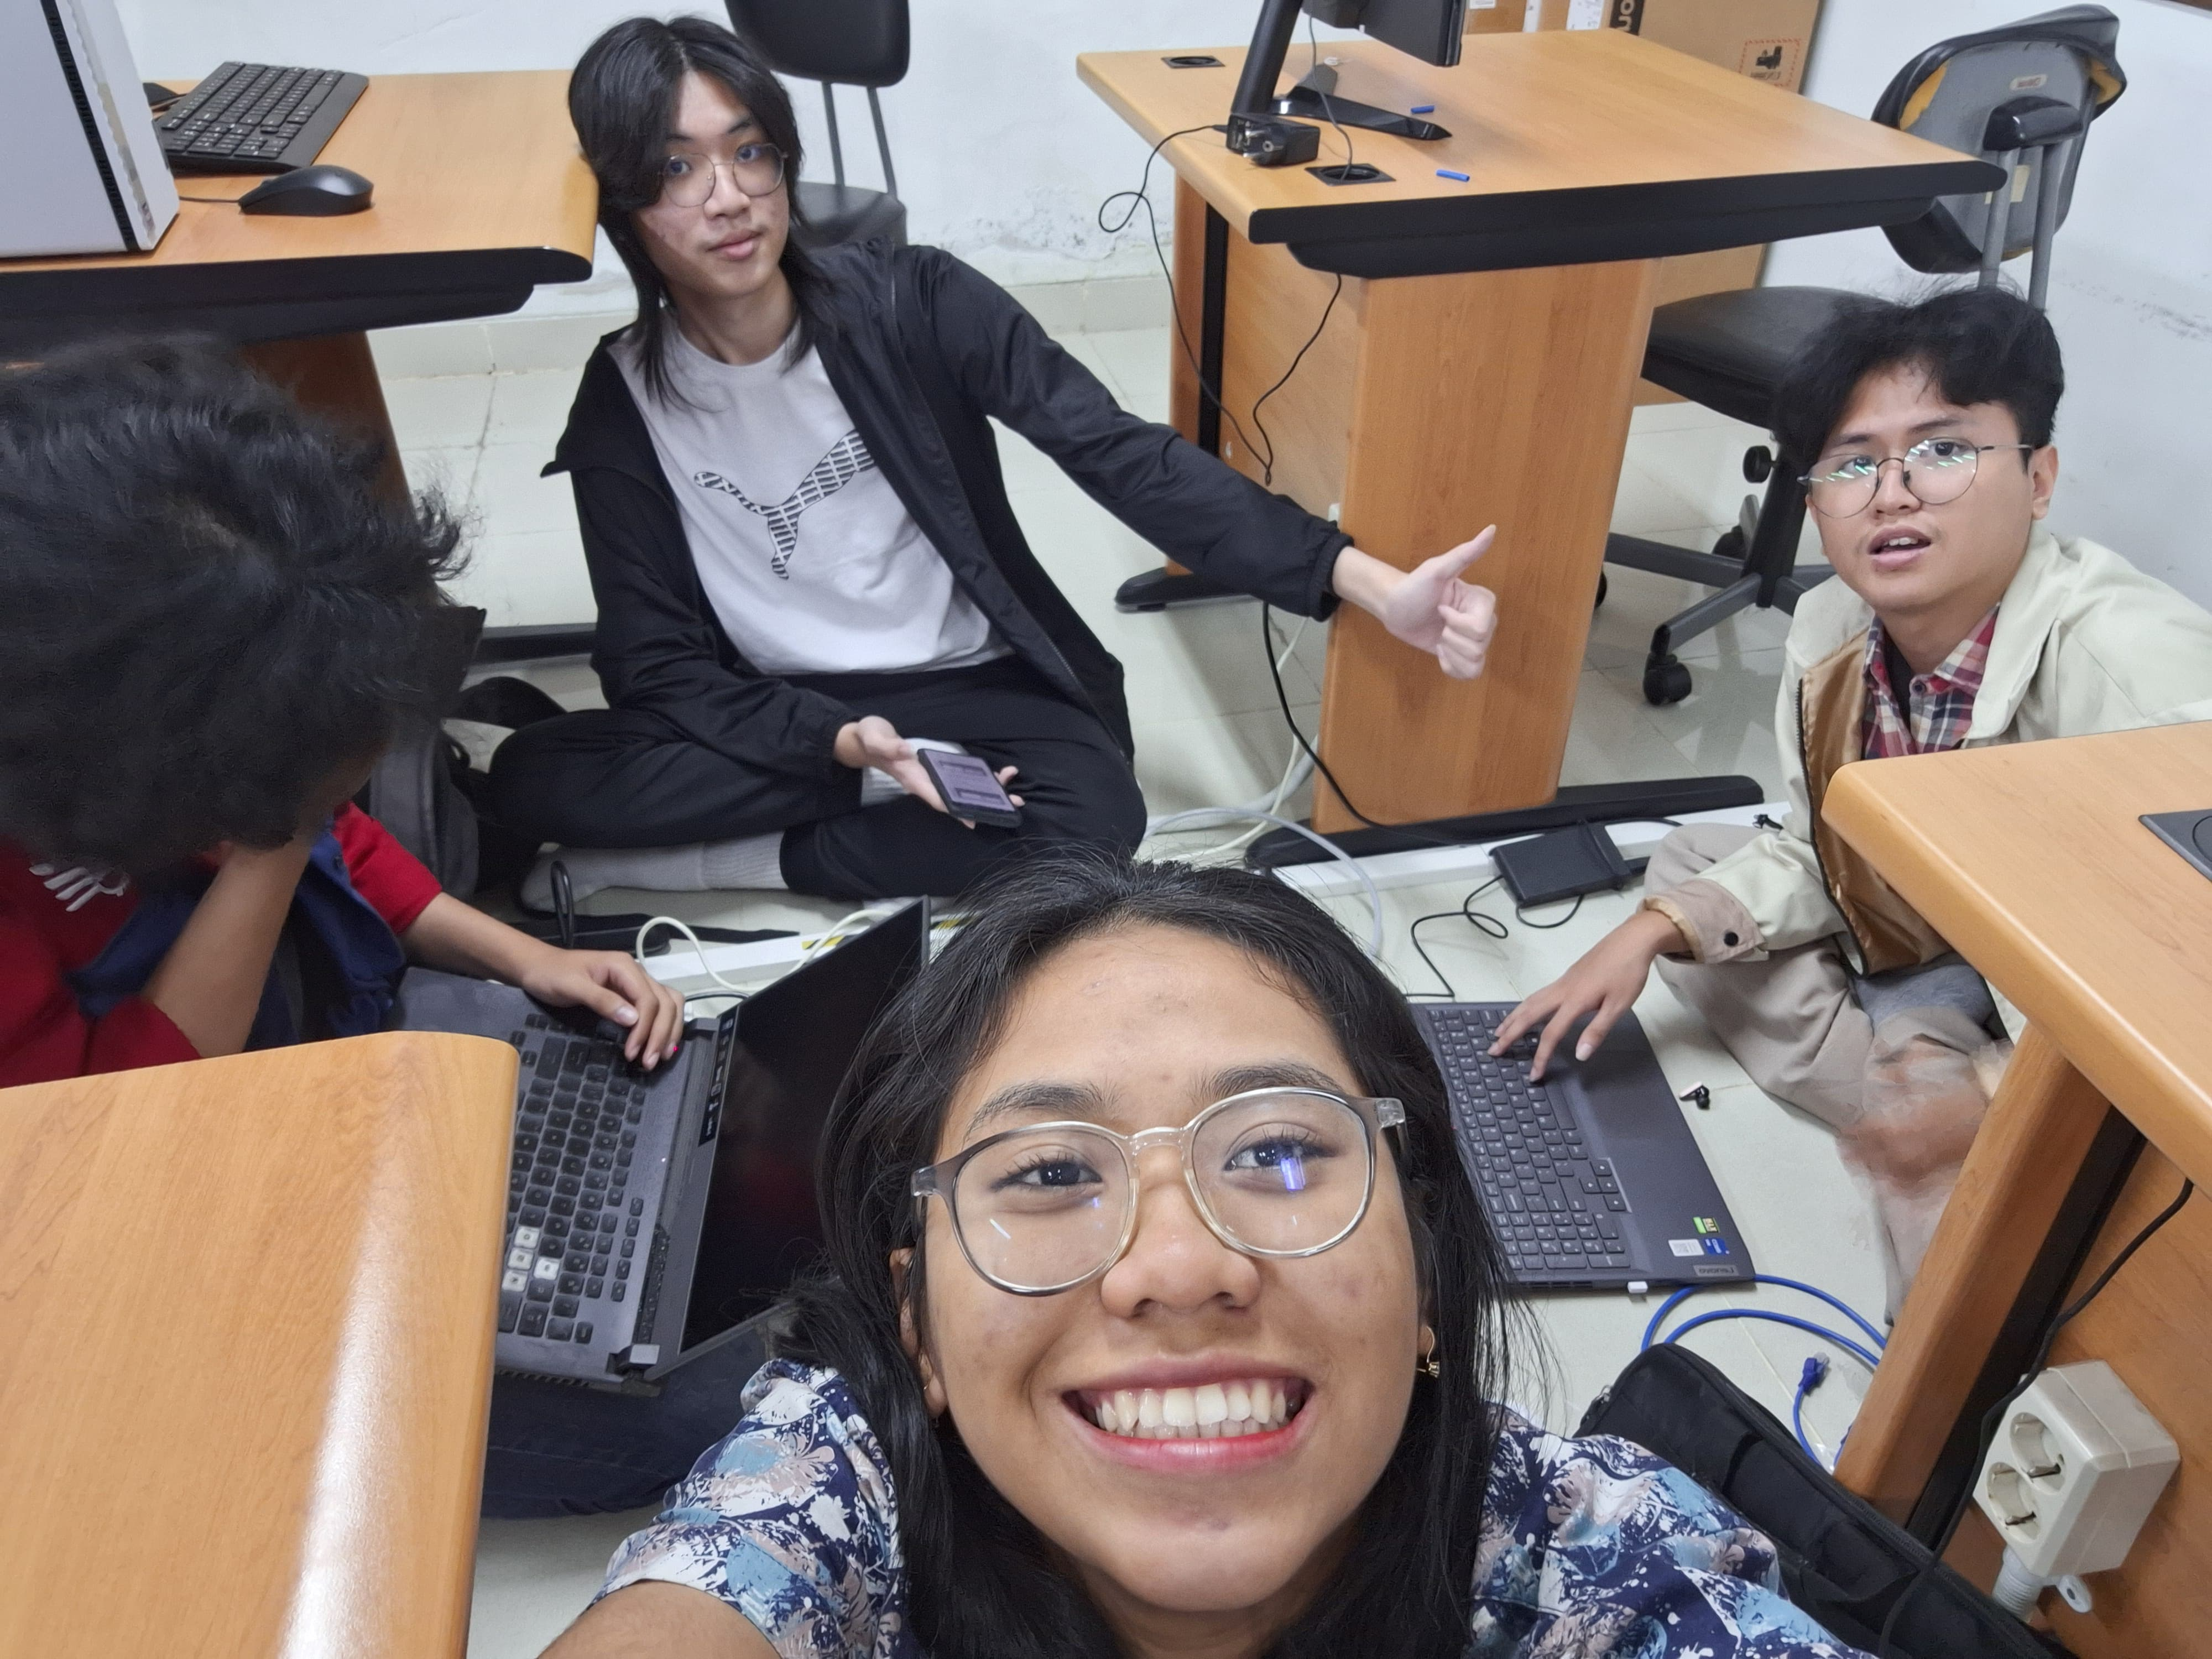
\includegraphics[scale=0.1]{P1/img/komunal 1.jpg}
        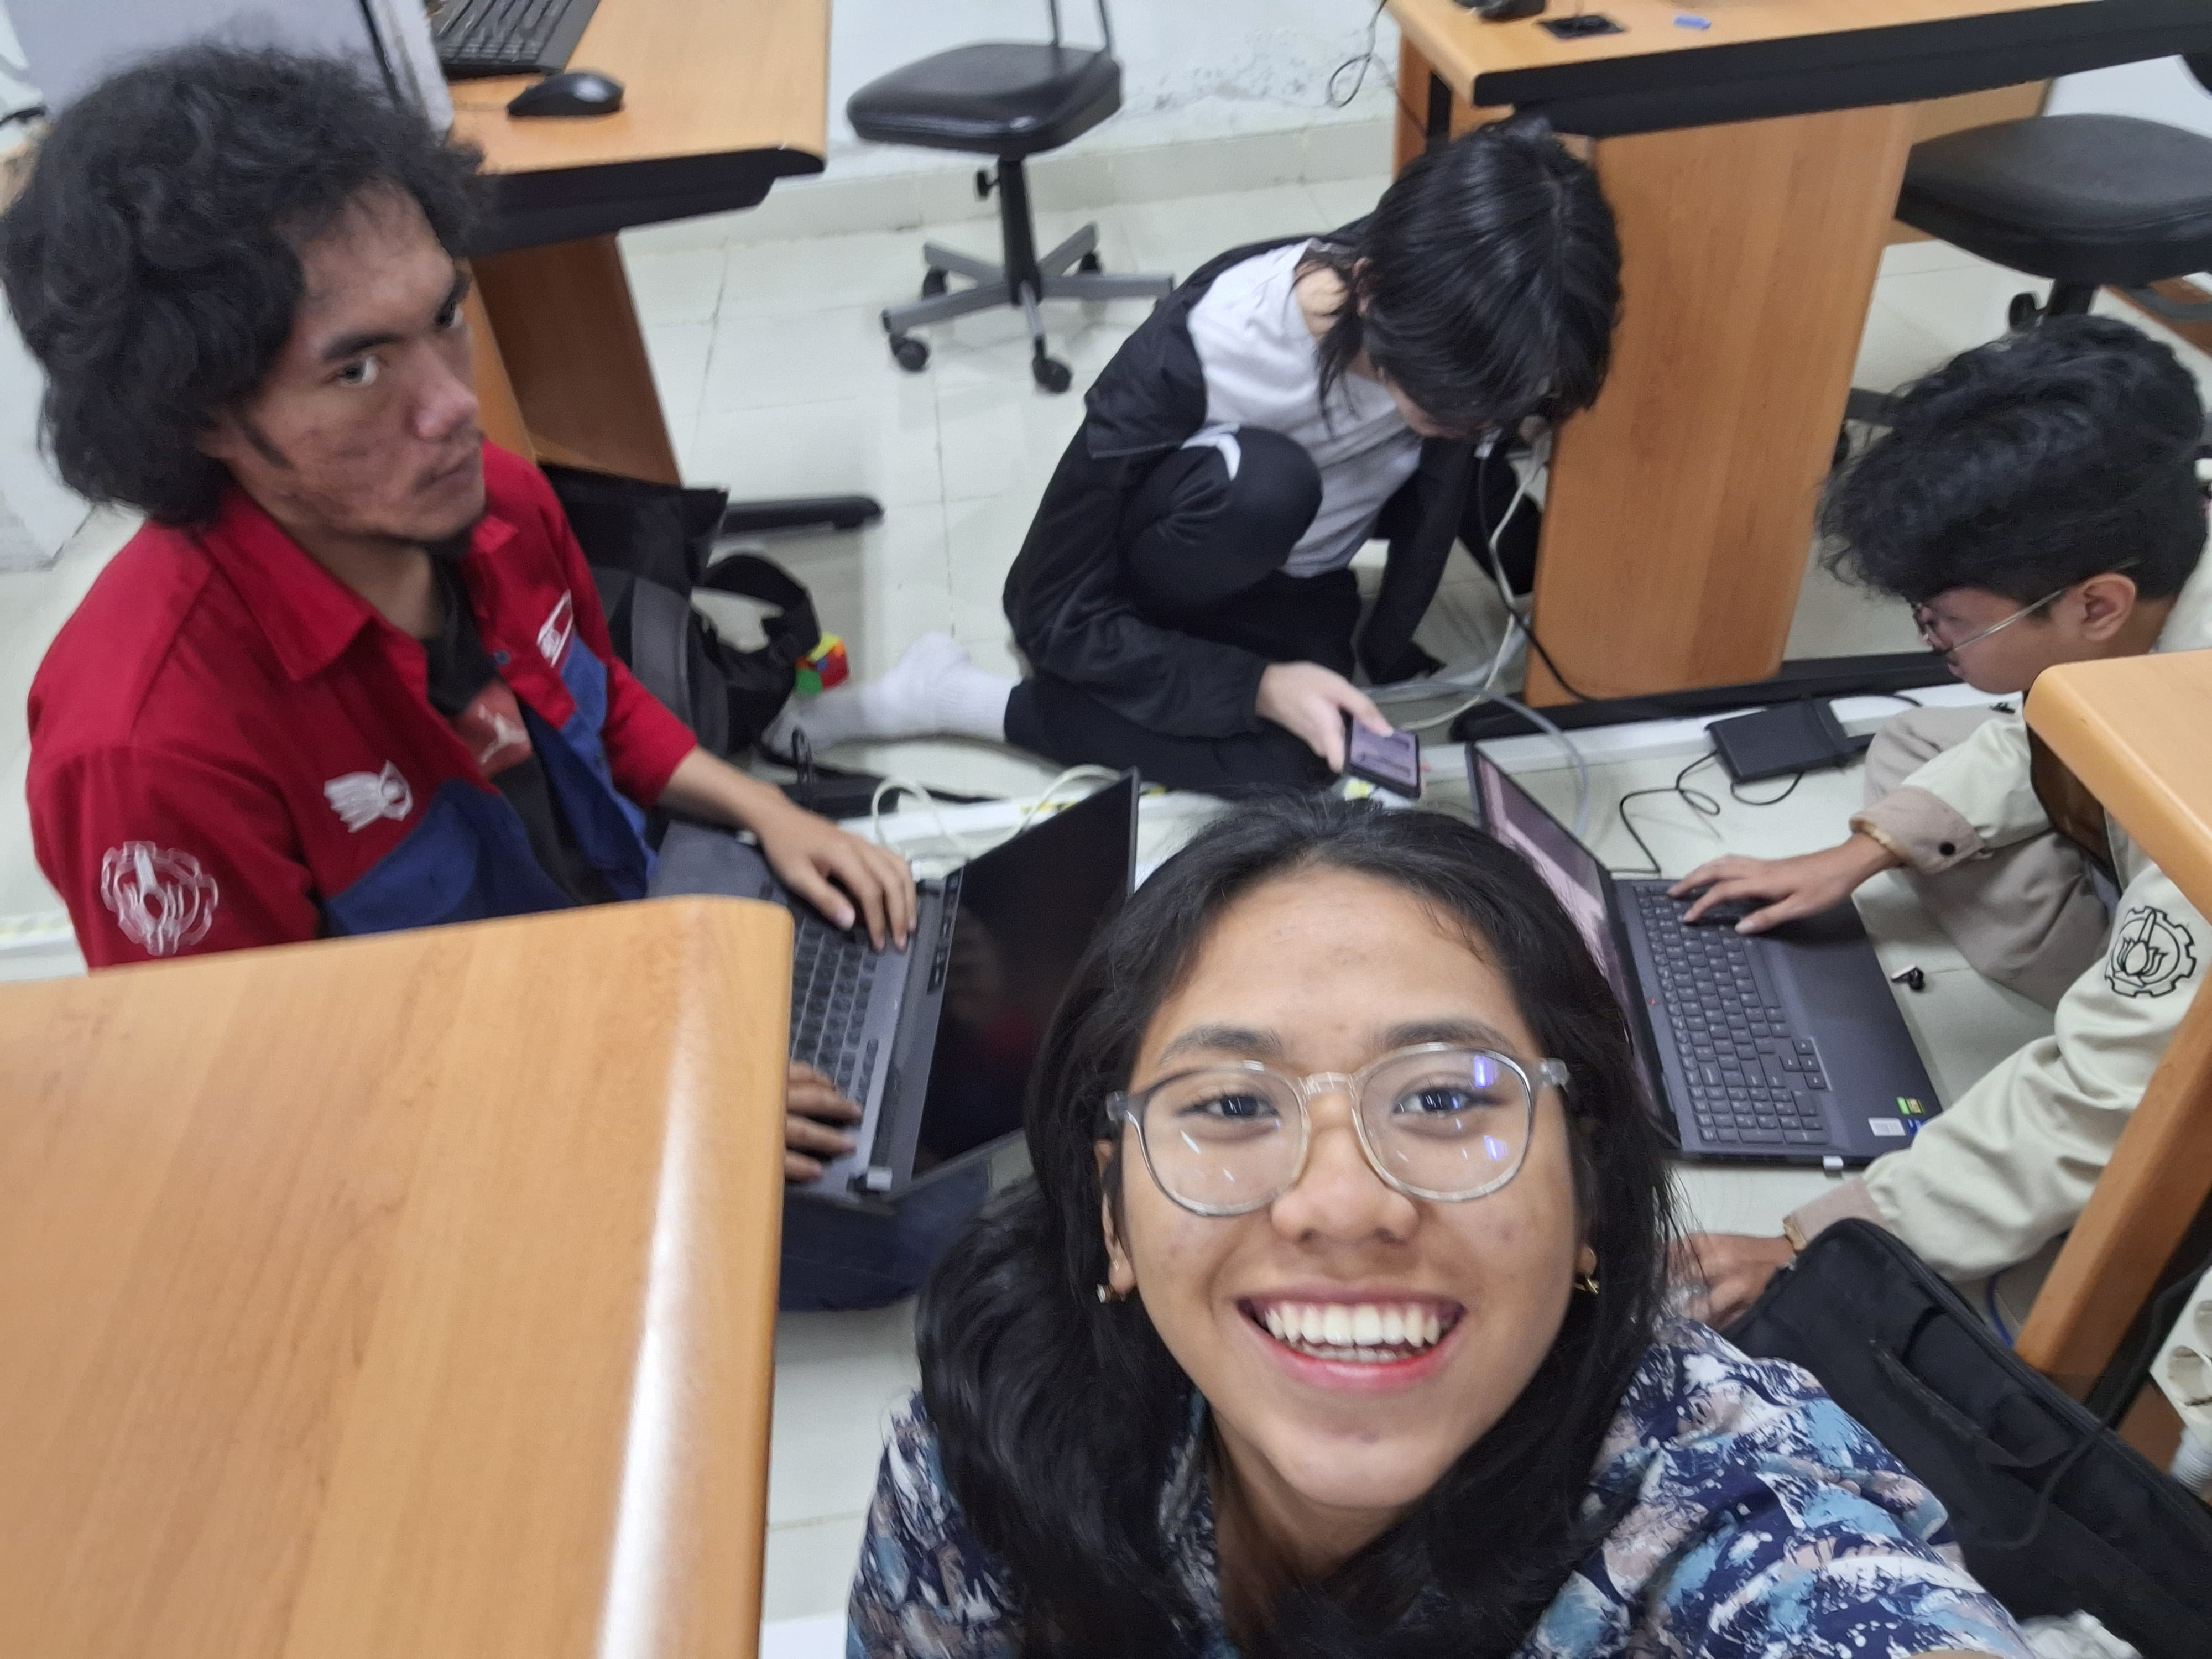
\includegraphics[scale=0.1]{P1/img/komunal 2.jpg}        
    \end{center}

\end{document}